\documentclass[10pt]{article}

% Pacotes extras necessários
\usepackage{amsmath}
\usepackage[lmargin=0.5in, rmargin=0.5in, tmargin=0.5in, bmargin=0.5in, includehead, includefoot]{geometry}
\usepackage{amsfonts}
\usepackage[utf8]{inputenc}
\usepackage[portuguese]{babel}
\usepackage{graphicx}
\usepackage{fancyhdr}
\usepackage{setspace}
\usepackage{listings}
\usepackage{url}
\usepackage{enumitem}
\usepackage{appendix} % For creating appendix sections

% More defined colors
\usepackage[dvipsnames]{xcolor}

% Define a custom style for the code listing
\lstdefinestyle{mystyle}{
    language=Octave,
    backgroundcolor=\color{white},   % Choose the background color
    basicstyle=\ttfamily\footnotesize, % Set the font and size for the code
    numbers=left,                    % Line numbers on the left
    numberstyle=\tiny\color{gray},   % Line numbers style
    numbersep=5pt,                   % Distance of line numbers from the code
    tabsize=2,                       % Set tab size (default is 8 spaces)
    breaklines=true,                 % Automatically wrap long lines
    keywordstyle=\color{blue},       % Keywords in blue
    commentstyle=\color{green!60!black}, % Comments in green
    stringstyle=\color{orange},      % Strings in orange
    frame=single,                    % Draw a frame around the code
    keepspaces=true,                 % Preserve spaces in text
    showspaces=false,                % Don't show spaces in strings
    showstringspaces=false,          % Don't show spaces in strings
    showtabs=false,                  % Don't show tabs in strings
    % Add any other options you need
}

\lstset{style=mystyle} % Set the custom style
 
% Required package
\usepackage{tikz}
\usetikzlibrary{positioning}

\graphicspath{ {./images/} }

% Sets para outras partes
\setlength{\parindent}{0pt}
\setstretch{1.5}
\DeclareMathOperator{\sen}{sen}
\DeclareMathOperator{\sinc}{sinc}

%% Facilidades
%% -- Laplace
\newcommand{\Lap}[1]{\mathcal{L}\left\{#1\right\}}

%% -- Negrito em matemáticas
\newcommand{\bm}[1]{\boldsymbol{#1}}


% ------- Estilo do trabalho -------- %
\fancypagestyle{capa}{
    \fancyhf{}
    \renewcommand\headrulewidth{0pt}
}

\pagestyle{fancy}
\fancyhead{}
\fancyhead[L]{\thepage}
\fancyfoot{}
% ----------------------------------- %

% Dados do Grupo
\title{Modelagem de Sistemas Dinâmicos - Trabalho Nº4}
\author{
    Leonardo Soares da Costa Tanaka - DRE: 121067652 \\
    Engenharia de Controle e Automação/UFRJ \\
    Rio de Janeiro, Brasil \\
    Julho de 2023
}
\date{}

\begin{document}
\maketitle
\thispagestyle{capa}

\quad Para este trabalho, vamos utilizar o arquivo “trabalho4-2023-1.mat” que tem os sinais de entrada u(t) e de saída y(t) de um sistema
linear contínuo com função de transferência G(s). Os sinais u e y foram aplicados e aquisitados
com uma frequência de amostragem fs = 2Hz (período de amostragem T = 0.5s). A variável
independente tempo t é o vetor com os instantes que foram realizadas as amostragens dos
sinais u(t) e y(t).

\quad Vale notar que o sinal de saída y(t) está quantizado e contaminado com ruído.

\section{FFT}

\quad Determinando, utilizando a FFT (Fast Fourier Transform), o espectro do sinal de entrada
(módulo e fase) em função da frequência em Hz. Utilizando Python e as bibliotecas disponíveis
(NumPy, Matplotlib e Scipy) que auxiliam na utilização da FFT, na plotagem dos espectros e
na coleta dos dados do arquivo .mat.

\begin{figure}[h]
    \centering
    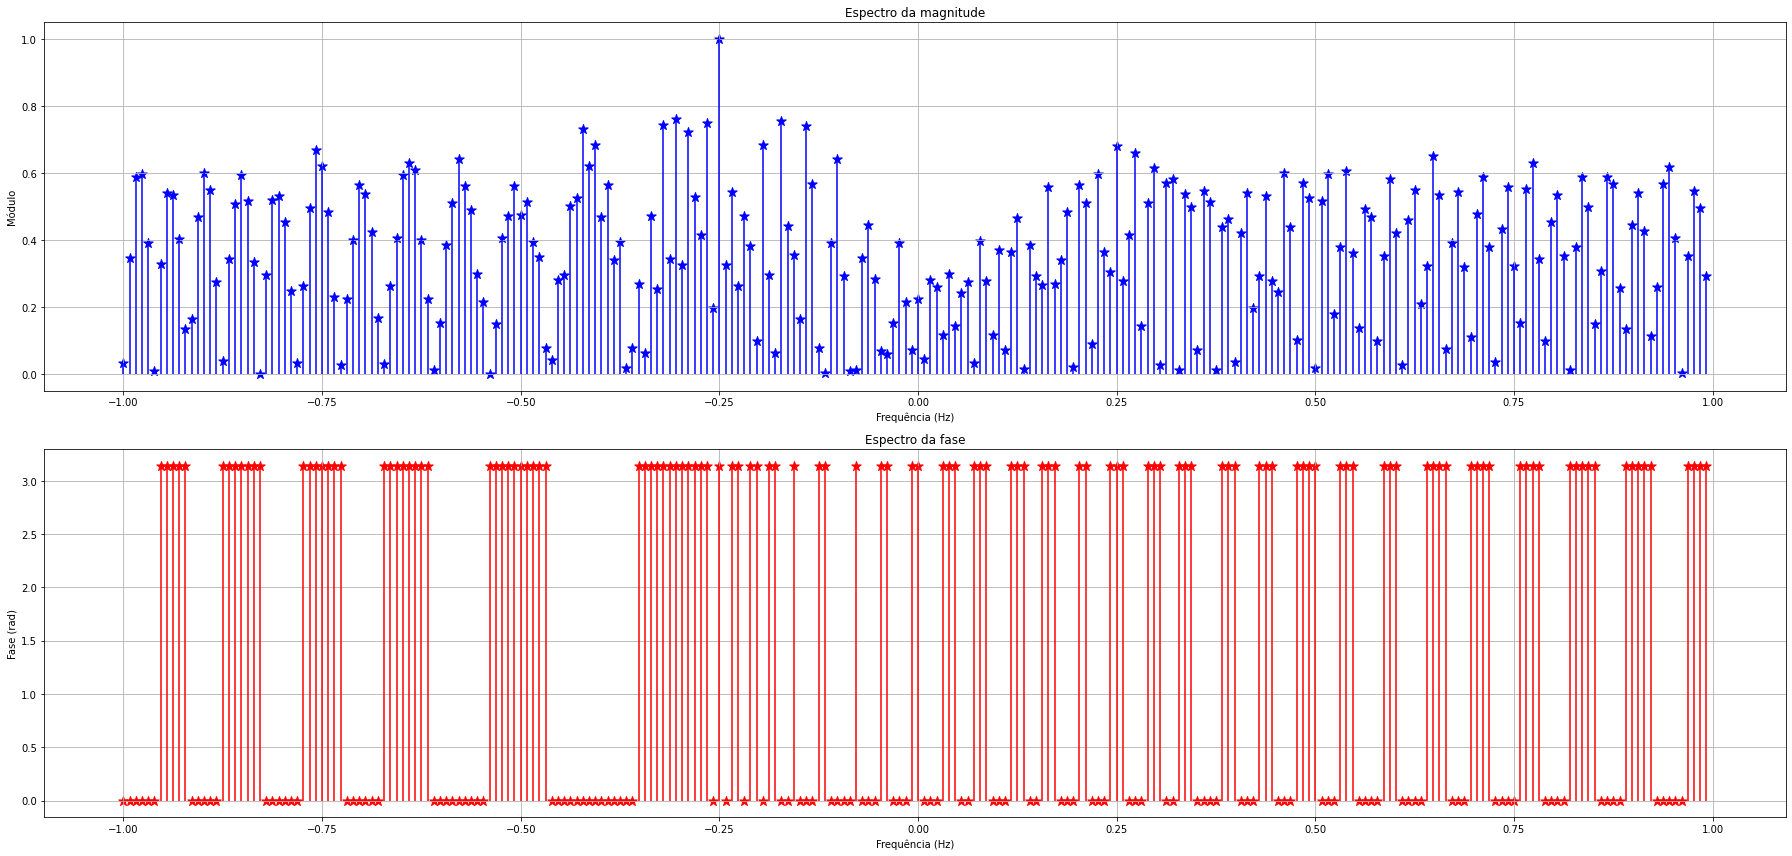
\includegraphics[scale=0.27]{fft.png}
    \caption{Espectros dos sinais da entrada}
\end{figure}

\quad É possível observar a magnitude que varia entre 0 e 1
com uma maior concentração de amostras abaixo de 0.6,
um padrão de oscilação mais lento na parte esquerda do espectro e
um padrão de oscilaçãõ mais rápido na parte direita do espectro.
Já no espectro de fase, os valores ficaram variando entre dois valores 0 e $\pi$
com um padrão de oscilação mais lento na parte esquerda do espectro e
um padrão de oscilaçãõ mais rápido na parte direita do espectro.

\small
\begin{verbatim}
    # Importando as bibliotecas
    import numpy as np
    import matplotlib.pyplot as plt
    from scipy.io import loadmat
    data = loadmat('trabalho4-2023-1.mat') # Carregar os dados do arquivo
    u = np.array(data['u'])
    y = np.array(data['y'])
    t = np.array(data['t'])
    # Frequencia de amostragem (fs) e período de amostragem (T)
    fs = 2  # Hz
    T = 1 / fs
    U = np.fft.fft(u) # Calcula o espectro do sinal de entrada u(t) usando a FFT
    frequencies = np.fft.fftfreq(len(U), d=T) # Vetor de frequencias para o eixo x
    modulo_U = np.abs(U) # Modulo do espectro do sinal de entrada
    fase_U = np.angle(U) # Fase do espectro do sinal de entrada
    # Plot do espectro do sinal de entrada (módulo e fase)
    plt.figure(figsize=(25, 12))
    # Plot do modulo com estrelas e linhas para o eixo x
    plt.subplot(2, 1, 1)
    plt.scatter(frequencies, modulo_U, marker='*', s=100, color='b')
    plt.vlines(frequencies, ymin=0, ymax=modulo_U, colors='b')
    plt.xlabel('Frequencia (Hz)')
    plt.ylabel('Módulo')
    plt.title('Espectro da magnitude')
    plt.grid()
    # Plot da fase com estrelas e linhas para o eixo x
    plt.subplot(2, 1, 2)
    plt.scatter(frequencies, fase_U, marker='*', s=100, color='r')
    plt.vlines(frequencies, ymin=0, ymax=fase_U, colors='r')
    plt.xlabel('Frequencia (Hz)')
    plt.ylabel('Fase (rad)')
    plt.title('Espectro da fase')
    plt.grid()
    plt.tight_layout()
    plt.show()
\end{verbatim}

\section{Resposta em frequência do sistema G(jw)}

\quad Estimando a resposta em frequência do sistema G(jw) utilizando os espectros dos sinais
de entrada U(jw) e de saída Y(jw):

\begin{figure}[h]
    \centering
    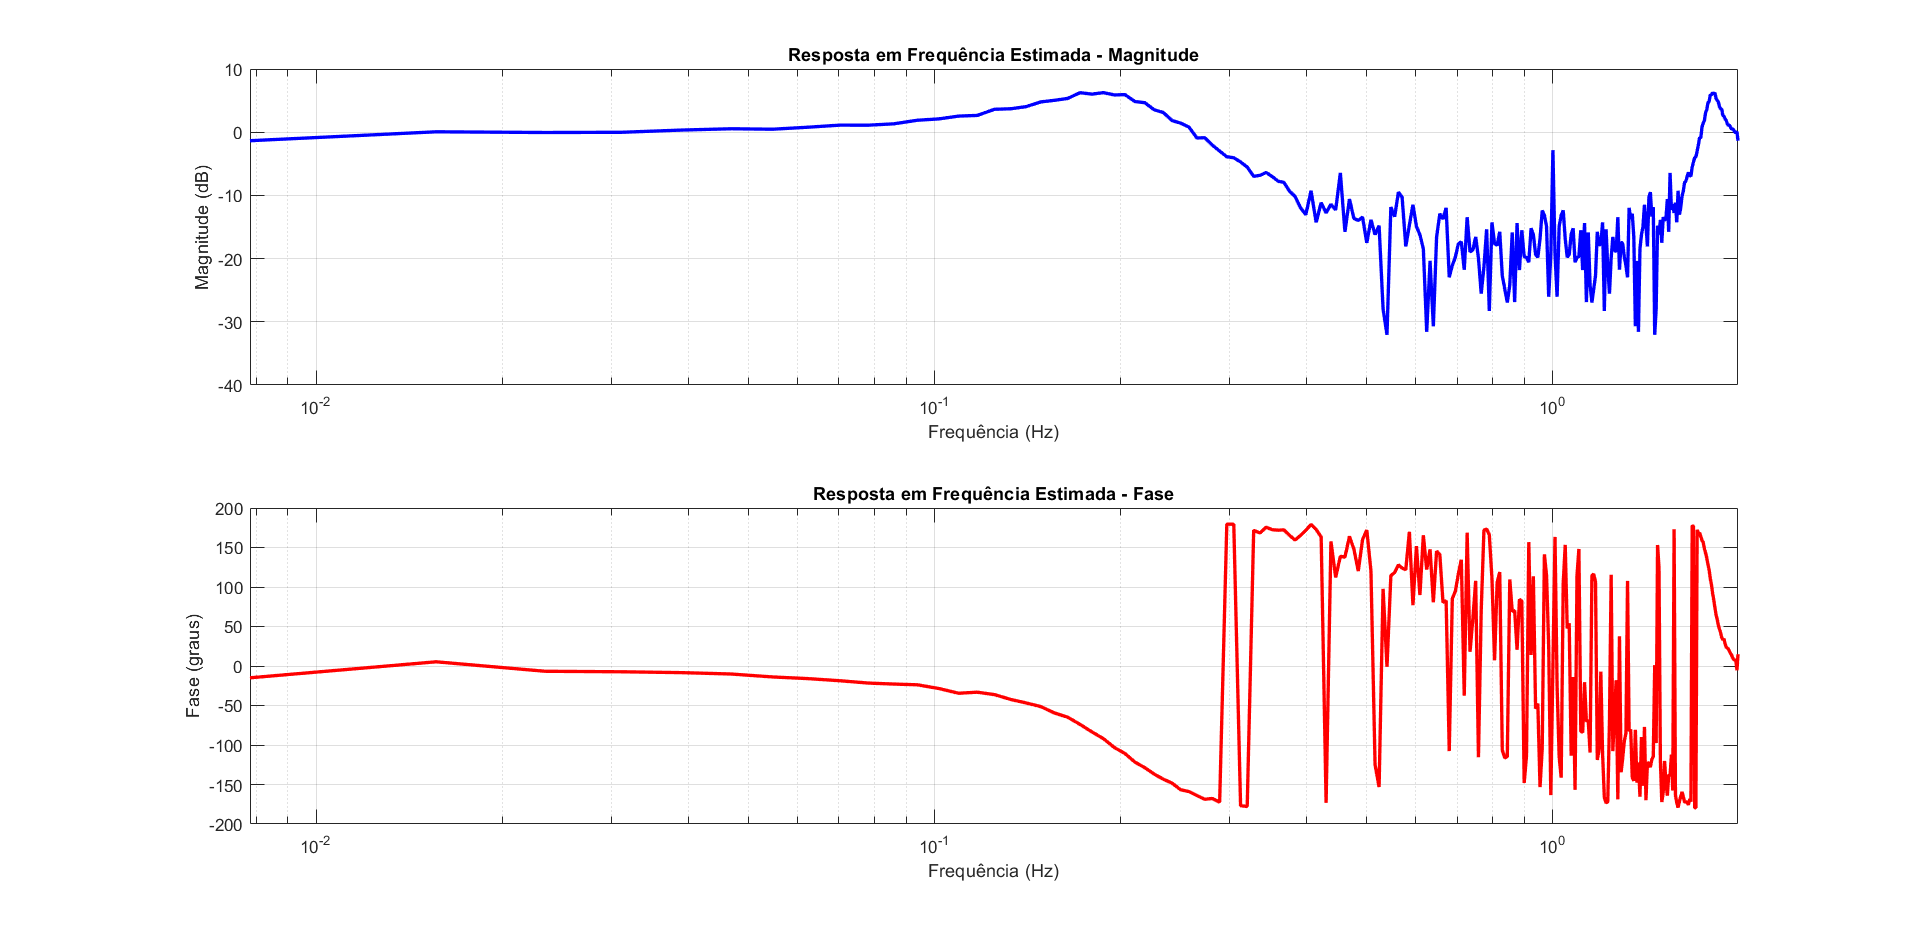
\includegraphics[scale=0.26]{g.png}
    \caption{Resposta em frequência}
\end{figure}

\small
\begin{verbatim}
    Y = np.fft.fft(y) # Calcula o espectro do sinal de saida y(t) usando a FFT
    G = Y / U # Calcula a resposta em frequencia estimada G(jw)
    modulo_G_dB = 20 * np.log10(np.abs(G)) # Calcula o modulo em dB da resposta em frequencia estimada
    fase_G_graus = np.angle(G) * (180 / np.pi) # Calcula a fase em graus da resposta em frequencia estimada
    plt.figure(figsize=(25, 12)) # Plot dos graficos usando subplot
    plt.subplot(2, 1, 1) # Plot do modulo com estrelas e linhas para o eixo x (resposta em frequencia estimada - modulo)
    plt.scatter(frequencies, modulo_G_dB, marker='*', s=100, color='b')
    plt.vlines(frequencies, ymin=0, ymax=modulo_G_dB, colors='b', linestyles='dotted')
    plt.xlabel('Frequencia (Hz)')
    plt.ylabel('Modulo da Resposta em Frequencia (dB)')
    plt.title('Resposta em Frequencia Estimada')
    plt.grid()
    plt.subplot(2, 1, 2) # Plot da fase com estrelas e linhas para o eixo x (resposta em frequencia estimada - fase)
    plt.scatter(frequencies, fase_G_graus, marker='*', s=100, color='r')
    plt.vlines(frequencies, ymin=0, ymax=fase_G_graus, colors='r', linestyles='dotted')
    plt.xlabel('Frequencia (Hz)')
    plt.ylabel('Fase da Resposta em Frequencia (graus)')
    plt.title('Fase da Resposta em Frequencia Estimada')
    plt.grid()
    plt.tight_layout()
    plt.show()
\end{verbatim}

\end{document}